\section{Лекция 5}
 
\subsection{Нормальня форма Хомского (НФХ)}

\begin{definition}
КС грамматика находится в нормальной форме Хомского если любое правило имеет один из трёх видов:
\begin{enumerate}
    \item $S \to \varepsilon$
    \item $N_i \to t_j$
    \item $N_i \to N_j N_k$, $N_j \neq S, N_k \neq S$
\end{enumerate}
\end{definition}
Важно: стартовый нетерминал не встречается в правых частях правил, $\varepsilon$-продукция только для стартового нетерминала.

\begin{note}
Любую КС грамматику можно преобразвать к нормальной форме Хомского.
\end{note}

Преобразование в НФХ. Шаги.
\begin{enumerate}
    \item Устранение длинных правил.
    \item Устранение $\varepsilon$-правил.
    \item Устранение цепных правил.
    \item Устранение бесполезных нетерминалов
    \begin{enumerate}
        \item Удаление непорождающих нетерминалов
        \item Удаление недостижимых нетерминалов
    \end{enumerate}
    \item Устранение продукций с правой частью длины 2, содержащей терминалы. 
\end{enumerate}

Надо не забыть добавить новый стартовый нетерминал, если нужно: чтобы вывести из него $\varepsilon$ и чтобы не встречался в правых частях правил. 

\textbf{Важно.}
Порядок применения шагов преобразования важен.
\begin{enumerate}
    \item Второй шаг можно поднять наверх, но это приведёт к более существенному разростанию результирующей граммтики.
    \item Подшаги шага 4 нельзя менять местами. Попробуйте поприменять их к граммтике:

\begin{align*}
S \to & A B \mid a \\
A \to & b
\end{align*}
    
\end{enumerate}

\href{https://neerc.ifmo.ru/wiki/index.php?title=%D0%9D%D0%BE%D1%80%D0%BC%D0%B0%D0%BB%D1%8C%D0%BD%D0%B0%D1%8F_%D1%84%D0%BE%D1%80%D0%BC%D0%B0_%D0%A5%D0%BE%D0%BC%D1%81%D0%BA%D0%BE%D0%B3%D0%BE}{Материалы по преобразованию в НФХ.}


\subsection{Лемма о накачке для КС языков}

\begin{theorem}
Пусть $L$ --- контекстно-свободный язык над алфавитом $\Sigma$, тогда существует такое $n$, что для любого слова $\omega \in L$, $|\omega| \geq n$ найдутся слова $u,v,x,y,z\in \Sigma^*$, для которых верно: $uvxyz = \omega, vy\neq \varepsilon,|vxy|\leq n$ и для любого $k \geq 0$  $uv^kxy^kz \in L$.
\end{theorem}

Идея доказательства леммы о накачке.

\begin{enumerate}
    \item Для любого КС языка можно найти грамматику в нормальной форме Хомского.
    \item Очевидно, что если брать достаточно длинные цепочки, то в дереве вывода этих цепочек, на пути от корня к какому-то листу обязательно будет нетерминал, встречающийся минимум два раза. Если $m$ --- количество нетерминалов в НФХ, то длины $2^{m+1}$ должно хватить. Это и будет $n$ из леммы.
    \item Возьмём путь, на котором есть хотя бы дважды повторяется некоторый нетерминал. Скажем, это нетерминал  $N_1$. Пойдём от листа по этому пути. Найдём первое появление $N_1$. Цепочка, задаваемая поддеревом для этого узла --- это $x$ из леммы.
    \item Пойдём дальше и найдём второе появление $N_1$. Цепочка, задаваемая поддеревом для этого узла --- это $vxy$ из леммы.
    \item Теперь мы можем копировать кусок дерева между этими повторениями $N_1$ и таким образом накачивать исходную цепочку.
\end{enumerate}

Надо только проверить выполение ограничений на длины.

\begin{figure}
\centering
\includegraphics[width=0.5\textwidth]{figures/pumping_tree_1.pdf}
\caption{Разбиение цепочки для леммы о накачке}
\label{fig:pumping1}
\end{figure}

\begin{figure}
\centering
\includegraphics[width=0.5\textwidth]{figures/pumping_tree_2.pdf}
\caption{Пример накачки цепочки с рисунка~\ref{fig:pumping1}}
\end{figure}


\href{https://neerc.ifmo.ru/wiki/index.php?title=%D0%9B%D0%B5%D0%BC%D0%BC%D0%B0_%D0%BE_%D1%80%D0%B0%D0%B7%D1%80%D0%B0%D1%81%D1%82%D0%B0%D0%BD%D0%B8%D0%B8_%D0%B4%D0%BB%D1%8F_%D0%9A%D0%A1-%D0%B3%D1%80%D0%B0%D0%BC%D0%BC%D0%B0%D1%82%D0%B8%D0%BA}{Материалы по лемме о накачке для КС языков.}

Проверить неконтекстно-свободность языка $L=\{a^nb^nc^n \mid n>0\}$.
